\chapter{Tetapan Kesetimbangan dan Pergeseran Kesetimbangan}\label{ch:b2:equilibrium-shifts}

Sebuah pabrik amonia menjalankan konverternya pada sekitar
\qty{450}{\celsius} dan \qty{200}{bar}. Pada suhu kamar, kesetimbangan
\ce{N2 + 3H2 <=>
2NH3} terletak begitu jauh di sisi amonia sehingga, pada
prinsipnya, campuran unsur-unsurnya dapat diubah hampir seluruhnya; namun
para insinyur memanaskannya, yang justru mendorong kesetimbangan mundur,
lalu memampatkannya sampai dua ratus atmosfer, yang memakan banyak sekali
energi. Alasannya adalah kompromi antara seberapa jauh sebuah reaksi dapat
berlangsung dan seberapa cepat reaksi itu berlangsung. Bab ini mengubah
\omterm{def:b2:reaction-free-energy:gibbs-energy}{energi Gibbs} dari bab-bab sebelumnya menjadi tetapan kesetimbangan dari
jilid Tahun 1, menunjukkan bagaimana tetapan itu berubah terhadap suhu,
menghitung berapa banyak kondisi yang dapat dipilih secara bebas oleh
seorang peneliti, dan meramalkan ke arah mana sebuah kesetimbangan
bergeser ketika suhu, tekanan, atau komposisi diubah.

\begin{recall}
\Cref{ch:b2:reaction-free-energy}: kriteria evolusi
$\Delta_r G\,\dd\xi
\leq 0$ dan hubungan Gibbs--Helmholtz;
\cref{ch:b2:chemical-potential}: $\Delta_r G = \Delta_r G^\circ + RT\ln Q$.
Jilid Tahun 1: kuosien reaksi $Q = \prod_i a_i^{\nu_i}$, tetapan
kesetimbangan standar $K^\circ$ sebagai nilai $Q$ pada kesetimbangan,
hukum aksi massa, dan aturan ``$Q < K^\circ$: ke arah maju'', yang
semuanya dinyatakan di sana sebagai hukum; tabel kemajuan; keadaan akhir
satu atau dua reaksi. Jilid itu juga menjanjikan bahwa pilihan suhu dan
tekanan untuk amonia dan untuk belerang trioksida akan dijelaskan di sini.
\end{recall}

\begin{omfigure}
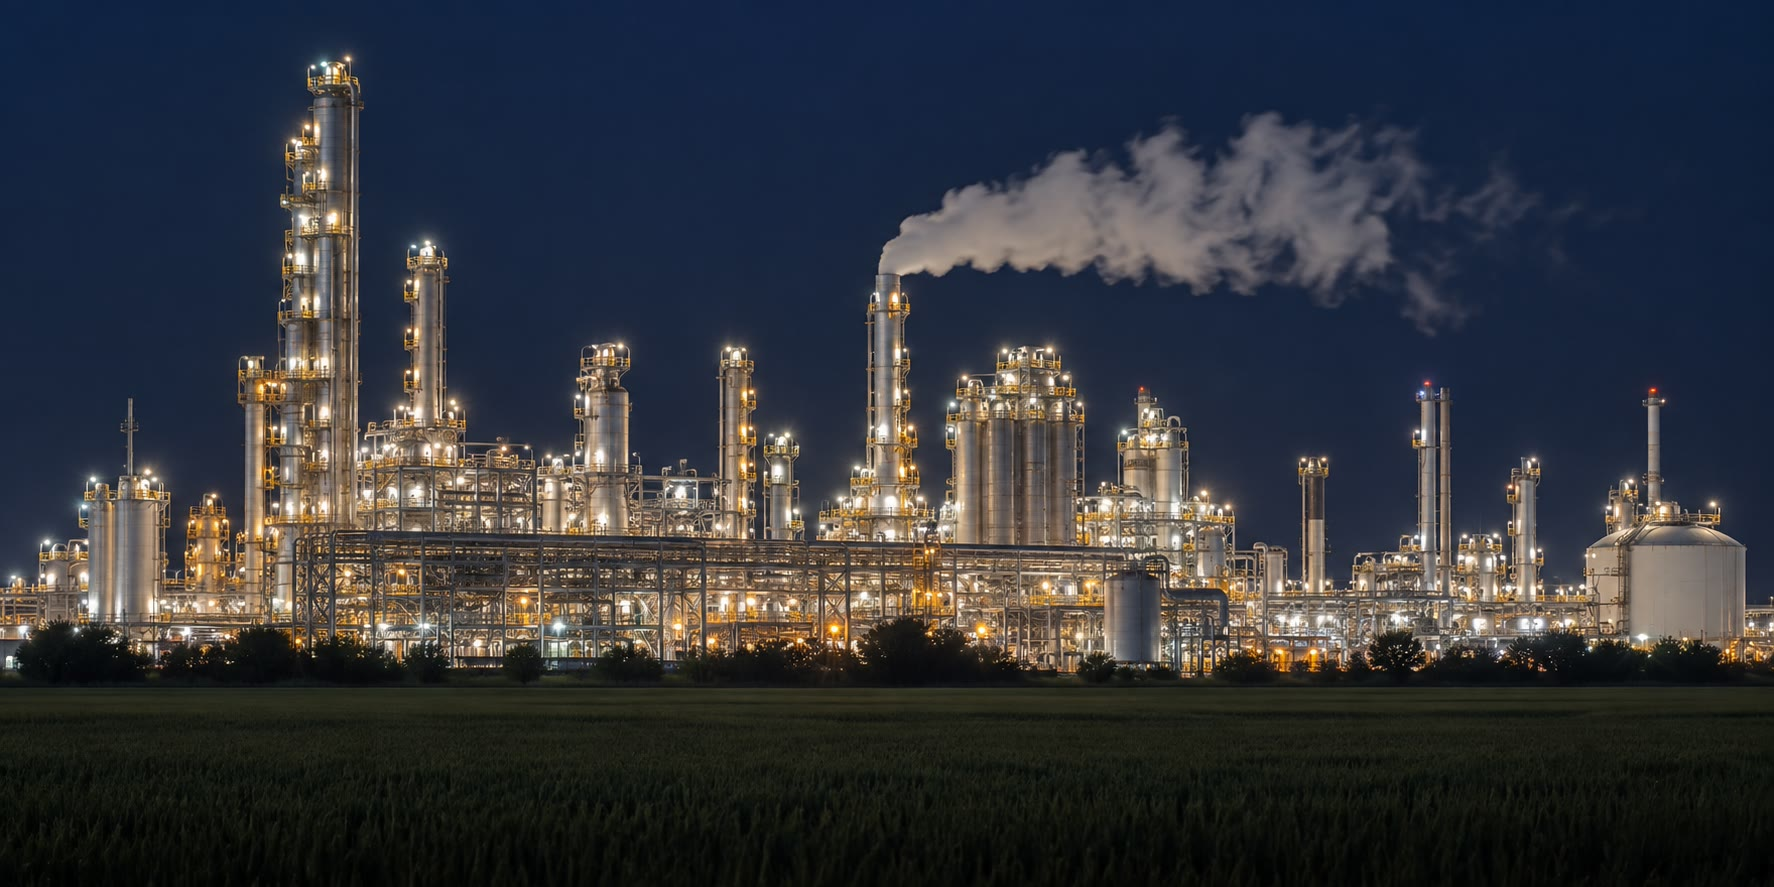
\includegraphics[width=0.7\linewidth]{images/book3/ai/b2-04-ammonia-plant.jpg}

{\small Sebuah pabrik amonia pada malam hari. Di dalam konverternya,
nitrogen dan hidrogen dialirkan melewati katalis besi pada suhu beberapa
ratus derajat dan tekanan beberapa ratus bar; pemilihan kondisi itu adalah
pokok bahasan soal akhir pekan.}
\end{omfigure}

\section{Tetapan kesetimbangan dari energi Gibbs}

\begin{theorem}[Tetapan kesetimbangan standar]\label{thm:b2:equilibrium-shifts:k-from-g}
Pada kesetimbangan $\Delta_r G = 0$, dan kuosien reaksi mencapai nilai
\[
  K^\circ(T) = \exp\!\left(-\frac{\Delta_r G^\circ(T)}{RT}\right), \qquad
  \Delta_r G^\circ(T) = -RT\ln K^\circ(T) .
\]
Tetapan ini hanya bergantung pada suhu.
\end{theorem}

\begin{proof}
Kriteria evolusi menjadikan $\Delta_r G = 0$ sebagai syarat kesetimbangan.
Dengan $\Delta_r G = \Delta_r G^\circ + RT\ln Q$
(\cref{prop:b2:chemical-potential:delta-g-q}), kesetimbangan berarti
$\ln Q_{\text{eq}}
= -\Delta_r G^\circ/(RT)$, yang merupakan fungsi $T$
saja karena $\Delta_r G^\circ$ demikian.
\end{proof}

\begin{corollary}[Hukum-hukum jilid Tahun 1]\label{cor:b2:equilibrium-shifts:mass-action}
$\Delta_r G = RT\ln(Q/K^\circ)$. Jadi sistem dengan $Q < K^\circ$
berevolusi ke arah maju, sistem dengan $Q > K^\circ$ ke arah balik, dan
sistem dengan $Q = K^\circ$ berada dalam kesetimbangan (hukum aksi massa).
\end{corollary}

\begin{proof}
Substitusikan $\Delta_r G^\circ = -RT\ln K^\circ$ ke dalam
$\Delta_r G = \Delta_r G^\circ
+ RT\ln Q$; tanda $\Delta_r G$ sama dengan
tanda $\ln(Q/K^\circ)$, dan kriteria evolusi mensyaratkan
$\Delta_r G\,\dd\xi \leq 0$.
\end{proof}

\begin{example}[Tiga tetapan pada \qty{298}{K}]\label{ex:b2:equilibrium-shifts:constants}
Sintesis amonia mempunyai $\Delta_r G^\circ = \qty{-32.8}{kJ/mol}$, sehingga
$K^\circ =
\exp(32\,800/(8.314 \times 298.15)) = \num{5.6e5}$ (tabel, dengan lebih
banyak angka, memberikan \num{5.4e5}). Disosiasi \ce{N2O4},
$\Delta_r G^\circ =
\qty{+4.7}{kJ/mol}$: $K^\circ = 0.15$. Penguraian batu
kapur, $\Delta_r G^\circ = \qty{+130.4}{kJ/mol}$: $K^\circ = \num{1.5e-23}$,
dan tekanan kesetimbangan karbon dioksida di atas batu kapur pada suhu
kamar adalah $\num{1.5e-23}$ bar, praktis nol. Perubahan
\qty{5.7}{kJ/mol} pada $\Delta_r G^\circ$ pada \qty{298}{K} mengalikan
atau membagi $K^\circ$ dengan sepuluh.
% ledger: dfh:NH3_g, s0:NH3_g, janafG:NH3.298.15 (computed in figdata/bachelor-2/thermo-data.py and vant-hoff.py)
\end{example}

\omterm{def:b2:reaction-free-energy:gibbs-energy}{Energi Gibbs} seluruh sistem menunjukkan hal yang sama sebagai sebuah
lanskap: energi itu paling rendah pada kemajuan kesetimbangan, tempat
kemiringannya, $\Delta_r G$, sama dengan nol.

\begin{omfigure}
\begin{tikzpicture}
\begin{axis}[
  width=0.7\linewidth, height=5.6cm, xmin=0, xmax=1, ymin=-2.2, ymax=5.2,
  axis x line=bottom, axis y line=left, xlabel={kemajuan $\xi$ (mol)},
  ylabel={$G(\xi) - G(0)$ (\unit{kJ})},
  tick label style={font=\small}, label style={font=\small}, clip=false]
\addplot[omDef, very thick] table[x=xi, y=G] {figdata/out/bachelor-2-gibbs-extent.dat};
\draw[dotted] (axis cs:0.189,-2.2) -- (axis cs:0.189,-0.949);
\fill[omThm] (axis cs:0.189,-0.949) circle (1.6pt);
\node[omThm, anchor=west, font=\small] at (axis cs:0.21,-1.75) {kesetimbangan, $\xi = 0.189$};
\draw[dashed, gray] (axis cs:0,0) -- (axis cs:1,4.728);
\node[gray, font=\scriptsize, anchor=south east] at (axis cs:1,4.75) {$\xi\,\Delta_r G^\circ$};
\end{axis}
\end{tikzpicture}

{\small \omterm{def:b2:reaction-free-energy:gibbs-energy}{Energi Gibbs} sistem tertutup berisi gas sempurna pada \qty{298}{K}
dan \qty{1}{bar}, mulai dari \qty{1}{mol} \ce{N2O4}, terhadap kemajuan
\ce{N2O4 <=> 2NO2}. Walaupun $\Delta_r G^\circ > 0$ (garis putus-putus,
spesies murni), pencampuran kedua gas menurunkan $G$, dan minimumnya
terletak pada $\xi =
0.189$, tempat $Q = K^\circ = 0.15$. Di sebelah
kirinya kemiringan $\Delta_r G =
\partial G/\partial\xi$ negatif, di
sebelah kanannya positif.}
% ledger: dfh:N2O4_g, s0:N2O4_g, dfh:NO2_g, s0:NO2_g (computed in figdata/bachelor-2/gibbs-extent.py)
\end{omfigure}

\section{Suhu: persamaan van 't Hoff}

\begin{theorem}[Persamaan van 't Hoff]\label{thm:b2:equilibrium-shifts:vant-hoff}
\[
  \frac{\dd\ln K^\circ}{\dd T} = \frac{\Delta_r H^\circ(T)}{RT^2}
\]
(\emph{persamaan van 't Hoff}\index{persamaan van 't Hoff}): tetapan
kesetimbangan reaksi \omterm{def:b2:reaction-enthalpy:exothermic}{endoterm} bertambah seiring kenaikan suhu, sedangkan
tetapan kesetimbangan reaksi \omterm{def:b2:reaction-enthalpy:exothermic}{eksoterm} berkurang.
\end{theorem}

\begin{proof}
Tuliskan $\ln K^\circ = -\Delta_r G^\circ/(RT)$ dan gunakan hubungan
Gibbs--Helmholtz pada \cref{prop:b2:reaction-free-energy:gibbs-helmholtz},
\[
  \frac{\dd}{\dd T}\left(\frac{\Delta_r G^\circ}{T}\right) =
  -\frac{\Delta_r H^\circ}{T^2} ;
\]
lalu bagilah dengan $-R$.
\end{proof}

\begin{proposition}[Bentuk terintegrasi]\label{prop:b2:equilibrium-shifts:integrated}
Jika $\Delta_r H^\circ$ tetap antara $T_1$ dan $T_2$ (\omterm{def:b2:reaction-free-energy:ellingham-approximation}{pendekatan
Ellingham}),
\[
  \ln\frac{K^\circ(T_2)}{K^\circ(T_1)} = -\frac{\Delta_r H^\circ}{R}\left(
  \frac{1}{T_2} - \frac{1}{T_1}\right),
\]
dan $\ln K^\circ$ merupakan garis lurus dengan kemiringan
$-\Delta_r H^\circ/R$ terhadap $1/T$.
\end{proposition}

\begin{proof}
Integrasikan $\dd\ln K^\circ = (\Delta_r H^\circ/R)\,\dd T/T^2$, dengan
memperhatikan bahwa $\dd T/T^2 = -\dd(1/T)$.
\end{proof}

\begin{omfigure}
\begin{tikzpicture}
\begin{axis}[
  width=0.72\linewidth, height=5.8cm, xmin=0.9, xmax=3.5, ymin=-19, ymax=15,
  axis x line=bottom, axis y line=left, xlabel={$1000/T$ (\unit{1/K})},
  ylabel={$\ln K^\circ$}, tick label style={font=\small},
  label style={font=\small}, clip=false]
\addplot[omThm, dashed, thick] table[x=invT, y=lnK] {figdata/out/bachelor-2-vant-hoff-a-line.dat};
\addplot[omDef, only marks, mark=*, mark size=1.8pt] table[x=invT, y=lnK] {figdata/out/bachelor-2-vant-hoff-a.dat};
\node[omDef, font=\scriptsize, anchor=west] at (axis cs:3.36,13.2) {\qty{298}{K}};
\node[omDef, font=\scriptsize, anchor=north west] at (axis cs:1.03,-15.3) {\qty{1000}{K}};
\node[omThm, font=\small, anchor=south east, align=right] at (axis cs:2.4,8) {kemiringan $-\Delta_r H^\circ(298)/R$\\ $= +11\,050$ K};
\end{axis}
\end{tikzpicture}

{\small Tetapan \ce{N2 + 3H2 <=> 2NH3} dari tabel (titik-titik, 298
sampai \qty{1000}{K}) dan garis van 't Hoff yang digambar dengan
$\Delta_r H^\circ$ pada \qty{298}{K} (putus-putus). Reaksi ini \omterm{def:b2:reaction-enthalpy:exothermic}{eksoterm}:
$K^\circ$ turun dari \num{5e5} menjadi \num{3e-7}. Pada suhu tinggi,
titik-titik itu jatuh di bawah garis: $\Delta_r H^\circ$ menjadi lebih
negatif ketika $T$ naik (\cref{ex:b2:reaction-enthalpy:kirchhoff}).}
% ledger: janafG:NH3.298.15, janafG:NH3.400, janafG:NH3.500, janafG:NH3.600, janafG:NH3.700, janafG:NH3.800, janafG:NH3.900, janafG:NH3.1000, dfh:NH3_g (computed in figdata/bachelor-2/vant-hoff.py)
\end{omfigure}

\begin{method}[Tetapan kesetimbangan pada suhu lain]\label{met:b2:equilibrium-shifts:k-at-t}
\begin{enumerate}
  \item Dari tabel pada \qty{298}{K}, hitunglah $\Delta_r H^\circ$,
        $\Delta_r
        S^\circ$, dan $K^\circ(298)$.
  \item Gunakan \omterm{thm:b2:equilibrium-shifts:vant-hoff}{persamaan van 't Hoff} terintegrasi, atau hitunglah
        $\Delta_r G^\circ(T) = \Delta_r H^\circ - T\Delta_r S^\circ$ lalu
        $K^\circ(T)$: keduanya merupakan pendekatan yang sama.
  \item Untuk selang yang lebar atau $\Delta_r C_p^\circ$ yang besar,
        utamakan $\Delta_f G^\circ(T)$ yang ditabelkan; galat
        \qty{5.7}{kJ/mol} pada \qty{298}{K} (atau \qty{13}{kJ/mol} pada
        \qty{700}{K}) berarti faktor sepuluh pada $K^\circ$.
\end{enumerate}
\end{method}

\begin{history}[Jacobus Henricus van 't Hoff]
\begin{minipage}[t]{0.2\linewidth}\vspace{0pt}
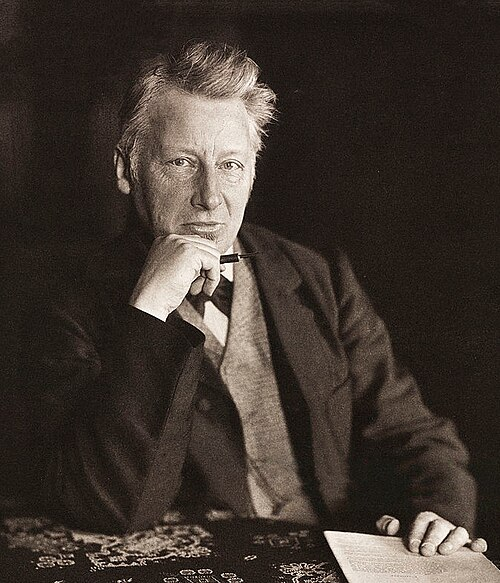
\includegraphics[width=\linewidth]{images/book3/vanthoff.jpg}
\end{minipage}\hfill
\begin{minipage}[t]{0.76\linewidth}\vspace{0pt}
Jacobus Henricus van 't Hoff (1852--1911) pada tahun 1884, dalam
\emph{Études de dynamique chimique}, memberikan hubungan antara suhu dan
tetapan kesetimbangan yang menyandang namanya, dan setahun kemudian hukum
\omterm{def:b2:chemical-potential:osmotic-pressure}{tekanan osmotik} pada \cref{ch:b2:chemical-potential}; sepuluh tahun
sebelumnya ia telah mengusulkan atom karbon tetrahedral. Ia menerima
Hadiah Nobel Kimia yang pertama, pada tahun 1901. (Foto oleh N.
Perscheid, 1904: domain publik, Wikimedia Commons.)
\end{minipage}
\end{history}

\section{Varians}

Berapa banyak besaran intensif yang dapat ditetapkan secara bebas oleh
seorang peneliti sebelum keadaan kesetimbangan tertentu sepenuhnya?

\begin{definition}[Varians]\label{def:b2:equilibrium-shifts:variance}
Yang disebut \emph{parameter intensif bebas}\index{parameter intensif bebas}
sebuah sistem dalam kesetimbangan adalah sekumpulan besaran intensif
(suhu, tekanan, fraksi mol dalam setiap fase) yang dapat dipilih secara
bebas dan yang, begitu dipilih, menetapkan semua besaran lainnya.
Banyaknya parameter itu disebut \emph{varians}\index{varians} $v$ sistem
(sering juga disebut derajat kebebasan sistem).
\end{definition}

\begin{theorem}[Aturan fase]\label{thm:b2:equilibrium-shifts:phase-rule}
Untuk sistem dengan $n$ spesies yang tersebar di antara $\varphi$ fase,
yang dihubungkan oleh $r$ reaksi kesetimbangan bebas dan oleh $s$
hubungan tambahan antara besaran-besaran intensif yang ditetapkan oleh
cara penyiapannya (umpan stoikiometris, kenetralan listrik),
\[
  v = c + 2 - \varphi, \qquad c = n - r - s .
\]
\end{theorem}

\begin{proof}
Variabel intensif: $T$, $p$, dan dalam setiap fase fraksi mol dari $n$
spesies, yang jumlahnya 1, sehingga ada $n - 1$ yang bebas per fase: seluruhnya
$2 +
\varphi(n - 1)$. Hubungan: setiap spesies berada dalam kesetimbangan
di antara fase-fase, yaitu $\varphi - 1$ kesamaan \omterm{def:b2:chemical-potential:chemical-potential}{potensial kimia} per
spesies, seluruhnya $n(\varphi -
1)$; setiap reaksi memberikan
$Q = K^\circ(T)$, yaitu $r$ hubungan; dan $s$ hubungan tambahan.
Kurangkan: $v = 2 + \varphi(n - 1) - n(\varphi - 1) - r -
s = n - r - s + 2 - \varphi$.
(Spesies yang tidak terdapat dalam suatu fase menghilangkan satu variabel
dan satu hubungan sekaligus.)
\end{proof}

\begin{method}[Menghitung varians]\label{met:b2:equilibrium-shifts:variance}
\begin{enumerate}
  \item Daftarlah spesies-spesiesnya, beserta fasenya, lalu hitunglah $n$
        dan $\varphi$ (setiap padatan murni adalah satu fase; semua gas
        membentuk satu fase).
  \item Hitunglah reaksi-reaksi bebas $r$ di antara spesies itu.
  \item Hitunglah hubungan tambahan $s$: jumlah zat dalam perbandingan
        stoikiometris (hanya jika hubungan itu menyangkut besaran-besaran
        dalam fase yang sama), kenetralan listrik larutan ion.
  \item $v = n - r - s + 2 - \varphi$.
\end{enumerate}
\end{method}

\begin{example}[Tiga varians]\label{ex:b2:equilibrium-shifts:variances}
Batu kapur dalam bejana tertutup, \ce{CaCO3(s) <=> CaO(s) + CO2(g)}:
$n = 3$, $r =
1$, $\varphi = 3$ (dua padatan, satu gas): $v = 1$. Pilihlah
$T$, maka tekanan karbon dioksida sudah tertentu: $p = K^\circ(T)\,p^\circ$.
Campuran gas \ce{N2}, \ce{H2}, dan \ce{NH3} dalam kesetimbangan: $n = 3$,
$r = 1$, $\varphi = 1$, $v
= 3$ ($T$, $p$, dan satu variabel komposisi);
jika dibuat dari amonia saja, atau dari umpan stoikiometris, \ce{N2} dan
\ce{H2} berada dalam perbandingan 1 : 3, $s = 1$ dan $v = 2$: pada $T$ dan
$p$ tertentu, komposisinya sudah tertentu, seperti yang dipakai dalam soal
akhir pekan.
\end{example}

\section{Menggeser kesetimbangan}

\begin{definition}[Pergeseran kesetimbangan]\label{def:b2:equilibrium-shifts:shift}
Jika sebuah sistem dalam kesetimbangan diganggu (perubahan suhu, tekanan,
atau jumlah suatu zat), sistem itu pada umumnya tidak lagi berada dalam
kesetimbangan dan berevolusi menuju kesetimbangan baru. Yang disebut
\emph{pergeseran kesetimbangan}\index{pergeseran kesetimbangan} terjadi ke
arah maju jika reaksi itu maju ($\dd\xi > 0$) dan ke arah balik jika
tidak.
\end{definition}

\begin{method}[Meramalkan pergeseran]\label{met:b2:equilibrium-shifts:predict-shift}
Sesaat setelah gangguan, hitunglah (atau perkirakan tanda perubahan) $Q$
dan $K^\circ$. Jika sekarang $Q < K^\circ$, pergeseran terjadi ke arah
maju; jika $Q > K^\circ$, ke arah balik; jika kesamaannya masih berlaku,
tidak ada pergeseran.
\end{method}

\begin{omfigure}
\begin{tikzpicture}[font=\small, >={Stealth}]
  \draw[->, thick] (0,0) -- (11,0) node[right] {$\ln Q$};
  \draw[omThm, thick] (5.5,0.25) -- (5.5,-0.25) node[below, align=center] {$\ln K^\circ$\\ ($= \ln Q$ sebelumnya)};
  \fill (5.5,0) circle (2pt);
  \draw[omDef, thick] (2.8,0.25) -- (2.8,-0.25) node[below] {$\ln Q$ sesaat setelahnya};
  \draw[->, omDef, very thick] (3.0,0.6) -- (5.2,0.6) node[midway, above] {pergeseran maju};
  \draw[omProp, thick] (8.4,0.25) -- (8.4,-0.25) node[below] {$\ln Q$ sesaat setelahnya};
  \draw[->, omProp, very thick] (8.2,0.6) -- (5.8,0.6) node[midway, above] {pergeseran balik};
\end{tikzpicture}

{\small Gangguan menggeser $Q$ (atau $K^\circ$, jika suhunya berubah);
sistem kemudian bergeser sampai $Q = K^\circ$ lagi, ke arah maju jika $Q$
menjadi terlalu kecil, ke arah balik jika terlalu besar.}
\end{omfigure}

\begin{proposition}[Suhu]\label{prop:b2:equilibrium-shifts:temperature}
Pada tekanan tetap, menaikkan suhu menggeser kesetimbangan ke arah
\omterm{def:b2:reaction-enthalpy:exothermic}{endoterm} (ke arah maju jika $\Delta_r H^\circ > 0$), menurunkan suhu
menggesernya ke arah \omterm{def:b2:reaction-enthalpy:exothermic}{eksoterm}.
\end{proposition}

\begin{proof}
Pada komposisi dan tekanan tetap, $Q$ tidak berubah terhadap $T$ (untuk
sistem ideal); menurut van 't Hoff, $K^\circ$ bertambah seiring $T$ jika
$\Delta_r H^\circ >
0$. Jadi, sesaat setelah kenaikan $T$, $Q < K^\circ$:
ke arah maju.
\end{proof}

\begin{proposition}[Tekanan]\label{prop:b2:equilibrium-shifts:pressure}
Pada suhu dan komposisi tetap, menaikkan tekanan total sebuah
kesetimbangan fase gas menggesernya ke arah yang mengurangi jumlah molekul
gas (ke arah maju jika $\Delta\nu_{\text{gas}} < 0$). Jika
$\Delta\nu_{\text{gas}}
= 0$, tekanan tidak berpengaruh.
\end{proposition}

\begin{proof}
Dengan $p_i = x_ip$, $Q = \prod_i x_i^{\nu_i}\,(p/p^\circ)^{\Delta\nu_{\text{gas}}}$:
pada komposisi tetap, menaikkan $p$ mengalikan $Q$ dengan
$(p'/p)^{\Delta\nu_{\text{gas}}}$, yang $< 1$ jika
$\Delta\nu_{\text{gas}} <
0$. Maka $Q < K^\circ$: ke arah maju. Fase-fase
terkondensasi tidak menyumbang apa pun.
\end{proof}

\begin{proposition}[Menambahkan konstituen atau gas inert]\label{prop:b2:equilibrium-shifts:adding}
Penambahan sedikit konstituen gas $j$ pada kesetimbangan fase gas
mengubah $\ln Q$ sebesar
\[
  \left(\frac{\partial\ln Q}{\partial n_j}\right) = \frac{\nu_j}{n_j} -
  \frac{\Delta\nu_{\text{gas}}}{n_{\text{tot}}}\ \ \text{bila tetap: } T, p ;
  \qquad \frac{\nu_j}{n_j}\ \ \text{bila tetap: } T, V .
\]
Penambahan gas inert tidak berpengaruh pada volume tetap, dan pada
tekanan tetap berperan sebagai penurunan tekanan.
\end{proposition}

\begin{proof}
Pada $T$, $p$ tetap: $Q = \prod_i n_i^{\nu_i}\,(p/(p^\circ n_{\text{tot}}))^{
\Delta\nu_{\text{gas}}}$, yang turunan logaritmiknya terhadap $n_j$ adalah
$\nu_j/n_j - \Delta\nu_{\text{gas}}/n_{\text{tot}}$ (suku pertama nol
untuk gas inert, $\nu_j = 0$). Pada $T$, $V$ tetap: $p_i = n_iRT/V$ dan
$Q = \prod_i n_i^{
\nu_i}\,(RT/(p^\circ V))^{\Delta\nu_{\text{gas}}}$, yang
turunannya hanya $\nu_j/n_j$.
\end{proof}

\begin{remark}[Pereaksi yang ditambahkan justru mendorong reaksi mundur]\label{rem:b2:equilibrium-shifts:paradox}
Dalam sintesis amonia, $\nu(\ce{N2}) = -1$ dan $\Delta\nu_{\text{gas}} = -2$:
penambahan nitrogen pada $T$ dan $p$ tetap mengubah $\ln Q$ sebesar
$-1/n_{\ce{N2}} +
2/n_{\text{tot}}$, yang positif jika
$x(\ce{N2}) > 1/2$. Dalam campuran yang sudah kaya nitrogen, menambahkan
nitrogen lagi mengencerkan hidrogen sedemikian rupa sehingga amonia
terurai. Aturan ``menambahkan pereaksi mendorong reaksi maju'' aman pada
volume tetap, tetapi tidak selalu pada tekanan tetap.
\end{remark}

\begin{proposition}[Asas Le Chatelier]\label{prop:b2:equilibrium-shifts:le-chatelier}
Proposisi-proposisi di atas dirangkum oleh \emph{asas Le
Chatelier}\index{asas Le Chatelier}: sistem dalam kesetimbangan yang
diganggu suhu atau tekanannya bergeser ke arah yang melawan gangguan itu
(sistem menyerap kalor jika dipanaskan, mengurangi volume gasnya jika
dimampatkan).
\end{proposition}

\begin{proof}
Asas ini menyatakan kembali \cref{prop:b2:equilibrium-shifts:temperature}
(arah \omterm{def:b2:reaction-enthalpy:exothermic}{endoterm} menyerap kalor) dan \cref{prop:b2:equilibrium-shifts:pressure}
(molekul gas yang lebih sedikit menempati volume yang lebih kecil pada $T$
dan $p$ yang sama). Untuk penambahan materi pada tekanan tetap, asas ini
tidak dapat diandalkan (\cref{rem:b2:equilibrium-shifts:paradox}):
hitunglah $Q$.
\end{proof}

\begin{remark}[Ketika kesetimbangan berakhir]\label{rem:b2:equilibrium-shifts:rupture}
Pergeseran dapat berakhir bukan pada kesetimbangan baru, melainkan pada
hilangnya suatu fase. Jika dipanaskan dalam bejana tertutup, batu kapur
terurai sampai $p(\ce{CO2}) =
K^\circ(T)\,p^\circ$; jika jumlahnya tidak
cukup untuk mencapai tekanan itu, batu kapur habis seluruhnya dan $Q$
tetap di bawah $K^\circ$: sistem itu berada di luar kesetimbangan untuk
seterusnya, seperti yang sudah diamati dalam jilid Tahun 1.
\end{remark}

\begin{history}[Henry Le Chatelier]
\begin{minipage}[t]{0.2\linewidth}\vspace{0pt}
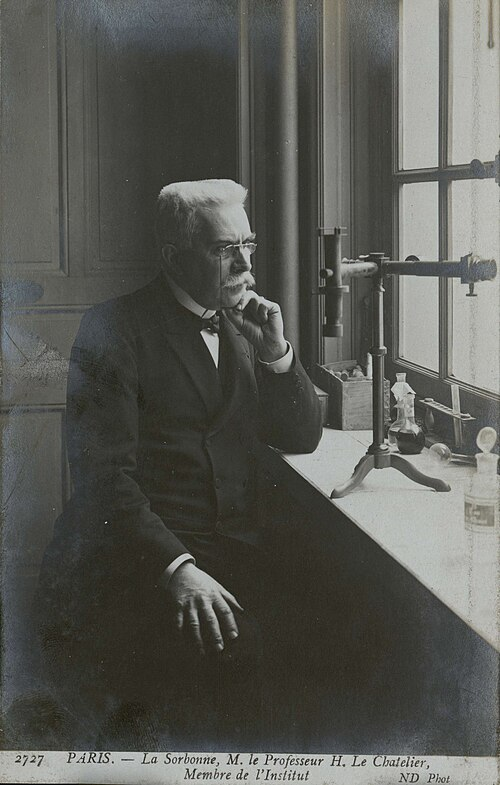
\includegraphics[width=\linewidth]{images/book3/lechatelier.jpg}
\end{minipage}\hfill
\begin{minipage}[t]{0.76\linewidth}\vspace{0pt}
Henry Le Chatelier (1850--1936), insinyur pertambangan dan kimiawan yang
meneliti semen, metalurgi, dan pirometri, pada tahun 1884 menyatakan
``hukum \omterm{def:b2:equilibrium-shifts:shift}{pergeseran kesetimbangan}'' yang menyandang namanya. Sekitar tahun
1901 ia juga telah mencoba membuat amonia dari unsur-unsurnya di bawah
tekanan; sebuah ledakan pada peralatannya mengakhiri upaya itu. (Foto:
penulis tidak diketahui, CC BY-SA 4.0, Wikimedia Commons.)
\end{minipage}
\end{history}

\section{Mengoptimalkan sebuah sintesis}

\subsection*{Amonia}

\begin{omfigure}
\begin{tikzpicture}
\begin{axis}[
  width=0.78\linewidth, height=6.2cm, xmin=500, xmax=1000, ymin=0, ymax=0.9,
  axis x line=bottom, axis y line=left, xlabel={$T$ (K)},
  ylabel={fraksi mol \ce{NH3} pada kesetimbangan},
  tick label style={font=\small}, label style={font=\small}, clip=false]
\addplot[omThm, very thick] table[x=T, y=p300] {figdata/out/bachelor-2-vant-hoff-b.dat};
\addplot[omDef, very thick] table[x=T, y=p200] {figdata/out/bachelor-2-vant-hoff-b.dat};
\addplot[omProp, very thick] table[x=T, y=p50] {figdata/out/bachelor-2-vant-hoff-b.dat};
\addplot[black!60, very thick] table[x=T, y=p1] {figdata/out/bachelor-2-vant-hoff-b.dat};
\node[omThm, font=\scriptsize, anchor=south west] at (axis cs:600,0.70) {300 bar};
\node[omDef, font=\scriptsize, anchor=north east] at (axis cs:612,0.52) {200 bar};
\node[omProp, font=\scriptsize, anchor=north east] at (axis cs:578,0.30) {50 bar};
\node[black!60, font=\scriptsize, anchor=south west] (onebar) at (axis cs:520,0.13) {1 bar};
\draw[black!60] (onebar.south west) -- (axis cs:512,0.075);
\draw[dotted] (axis cs:723,0) -- (axis cs:723,0.253);
\fill[omDef] (axis cs:723,0.253) circle (1.6pt);
\end{axis}
\end{tikzpicture}

{\small Fraksi mol amonia pada kesetimbangan dari campuran nitrogen dan
hidrogen 1 : 3 (gas sempurna), terhadap suhu pada empat tekanan, dihitung
dari \omterm{def:b2:reaction-free-energy:gibbs-energy}{energi Gibbs} yang ditabelkan. Tekanan menaikkannya, suhu
menurunkannya; titik menandai \qty{723}{K} dan \qty{200}{bar}.}
% ledger: janafG:NH3.500, janafG:NH3.600, janafG:NH3.700, janafG:NH3.800, janafG:NH3.900, janafG:NH3.1000 (computed in figdata/bachelor-2/vant-hoff.py)
\end{omfigure}

Sintesis ini \omterm{def:b2:reaction-enthalpy:exothermic}{eksoterm} dan mengurangi empat molekul gas menjadi dua:
menurut proposisi-proposisi di atas, suhu rendah dan tekanan tinggi
menguntungkan amonia. Pada \qty{1}{bar} dan suhu kamar, kesetimbangannya
hampir tuntas, tetapi reaksinya sama sekali tidak berjalan: ikatan rangkap
tiga nitrogen hanya putus pada permukaan katalis, dan katalis besi hanya
bekerja pada suhu beberapa ratus derajat. Karena itu pabrik memilih:
\begin{itemize}
  \item suhu yang cukup tinggi demi laju, serendah yang dimungkinkan oleh
        katalis (sekitar \qty{700}{K});
  \item tekanan tinggi untuk memulihkan rendemen yang hilang karena suhu,
        yang dibatasi oleh biaya pemampatan dan bejana berdinding tebal;
  \item sebuah sirkuit: gas yang keluar dari konverter didinginkan, amonia
        mengembun dan dipisahkan, dan gas yang tidak terkonversi didaur
        ulang bersama umpan segar; \omterm{def:b2:equilibrium-shifts:single-pass}{purge} kecil membuang argon dan metana
        yang jika tidak akan menumpuk.
\end{itemize}

\begin{definition}[Konversi sekali lewat, daur ulang, purge]\label{def:b2:equilibrium-shifts:single-pass}
Dalam proses dengan daur ulang, yang disebut \emph{konversi sekali
lewat}\index{konversi sekali lewat} adalah fraksi suatu pereaksi yang
terkonversi dalam satu kali lewat melalui reaktor; bagian yang tidak
terkonversi, setelah dipisahkan dari produk, dikembalikan ke saluran masuk
reaktor sebagai \emph{daur ulang}\index{daur ulang}; \emph{purge}\index{purge}
adalah aliran kecil yang terus-menerus diambil dari daur ulang untuk
mencegah spesies inert menumpuk.
\end{definition}

\begin{omfigure}
\begin{tikzpicture}[font=\small, >={Stealth}, box/.style={draw, thick, rounded corners=2pt, minimum width=2.1cm, minimum height=1.0cm, align=center, fill=white}]
  \node[box] (comp) at (0,0) {kompresor};
  \node[box] (conv) at (3.6,0) {konverter\\ (katalis)};
  \node[box] (cond) at (7.2,0) {pendingin dan\\ pemisah};
  \draw[->, thick] (-3.9,0) -- (comp) node[pos=0.0, above right] {\ce{N2 + 3H2} segar};
  \draw[->, thick] (comp) -- (conv);
  \draw[->, thick] (conv) -- (cond);
  \draw[->, thick, omDef] (cond.south) -- ++(0,-1.0) node[below] {amonia cair};
  \draw[->, thick, omThm] (cond.north) -- ++(0,0.9) -| (comp.north);
  \node[omThm, above] at (2.6,1.4) {daur ulang (gas tak terkonversi)};
  \draw[->, thick, black!60] (6.1,1.4) -- (6.1,2.1) node[above] {purge};
\end{tikzpicture}

{\small Sirkuit amonia. Setiap kali lewat hanya sebagian gas yang
terkonversi; amonia diembunkan dan dipisahkan, dan sisanya dimampatkan
kembali dan dikirim balik bersama umpan segar. \omterm{def:b2:equilibrium-shifts:single-pass}{Purge} mencegah argon dan
metana, yang tidak bereaksi, menumpuk.}
\end{omfigure}

\begin{history}[Haber dan Bosch]
\begin{minipage}[t]{0.15\linewidth}\vspace{0pt}
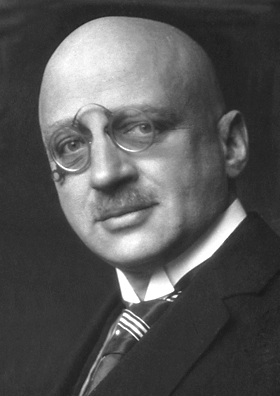
\includegraphics[width=\linewidth]{images/book3/haber.png}
\end{minipage}\hspace{0.01\linewidth}%
\begin{minipage}[t]{0.15\linewidth}\vspace{0pt}
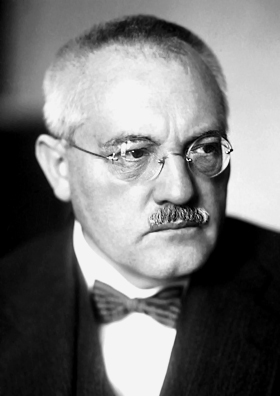
\includegraphics[width=\linewidth]{images/book3/bosch.jpg}
\end{minipage}\hfill
\begin{minipage}[t]{0.66\linewidth}\vspace{0pt}
Fritz Haber (1868--1934) mengukur kesetimbangan amonia di bawah tekanan
dan, pada tahun 1909, membuatnya mengalir terus-menerus dari konverter
laboratorium melewati katalis osmium. Carl Bosch (1874--1940) menjadikannya
sebuah industri, dengan bejana baja yang tahan terhadap hidrogen panas
bertekanan dan katalis besi yang murah; pabrik pertama mulai beroperasi
pada tahun 1913. Haber menerima Hadiah Nobel pada tahun 1918, Bosch pada
tahun 1931. (Potret dari Yayasan Nobel: domain publik, Wikimedia
Commons.)
\end{minipage}
\end{history}

\subsection*{Belerang trioksida}

Dalam proses kontak, \ce{2SO2(g) + O2(g) <=> 2SO3(g)} ($\Delta_r H^\circ =
\qty{-197.8}{kJ/mol}$ untuk persamaan sebagaimana tertulis) berlangsung di
atas katalis vanadium oksida, yang hanya aktif dalam keadaan panas, di
dalam beberapa unggun adiabatik. Dalam setiap unggun, kalor yang
dilepaskan menaikkan suhu, yang menurunkan $K^\circ$; konversi berhenti
ketika gas mencapai kurva kesetimbangan. Pendinginan di antara unggun
membawanya kembali ke suhu tempat kesetimbangan memungkinkan konversi
lebih lanjut.
% ledger: dfh:SO2_g, dfh:SO3_g

\begin{omfigure}
\begin{tikzpicture}
\begin{axis}[
  width=0.72\linewidth, height=6.4cm, xmin=600, xmax=900, ymin=0, ymax=1.08,
  axis x line=bottom, axis y line=left, xlabel={$T$ (K)},
  ylabel={konversi \ce{SO2}}, tick label style={font=\small},
  label style={font=\small}, clip=false]
\addplot[black, very thick] table[x=T, y=X] {figdata/out/bachelor-2-vant-hoff-c.dat};
\addplot[omThm, thick] table[x=T, y=X] {figdata/out/bachelor-2-vant-hoff-bed1.dat};
\addplot[omThm, thick] table[x=T, y=X] {figdata/out/bachelor-2-vant-hoff-bed2.dat};
\addplot[omThm, thick] table[x=T, y=X] {figdata/out/bachelor-2-vant-hoff-bed3.dat};
\draw[->, omDef, thick] (axis cs:892.8,0.676) -- (axis cs:712,0.676);
\draw[->, omDef, thick] (axis cs:784.4,0.924) -- (axis cs:712,0.924);
\node[font=\scriptsize, anchor=south west] at (axis cs:860,0.84) {kesetimbangan};
\node[omThm, font=\scriptsize, anchor=west] at (axis cs:800,0.24) {unggun 1 (adiabatik)};
\node[omDef, font=\scriptsize, anchor=south] at (axis cs:800,0.68) {pendinginan};
\end{axis}
\end{tikzpicture}

{\small Konversi kesetimbangan \ce{SO2} menjadi \ce{SO3} terhadap suhu
(hitam) untuk umpan model \qty{10}{\percent} \ce{SO2}, \qty{11}{\percent}
\ce{O2} pada \qty{1}{bar}, dan jalur gas melalui tiga unggun adiabatik
(merah, suhunya naik karena reaksi memanaskan gas), dengan pendinginan di
antara unggun (biru).}
% ledger: janafG:SO2.600, janafG:SO2.700, janafG:SO2.800, janafG:SO2.900, janafG:SO3.600, janafG:SO3.700, janafG:SO3.800, janafG:SO3.900 (computed in figdata/bachelor-2/vant-hoff.py; feed and adiabatic rise are model values)
\end{omfigure}

\section{Latihan}

\begin{exercise}[$\star$]\label{exo:b2:equilibrium-shifts:1}
Hitunglah $K^\circ$ pada \qty{298}{K} untuk reaksi dengan
$\Delta_r G^\circ =
\qty{-32.8}{kJ/mol}$, lalu untuk
$\Delta_r G^\circ = \qty{+32.8}{kJ/mol}$. Perubahan $\Delta_r G^\circ$
berapakah yang mengalikan $K^\circ$ dengan 100?
\end{exercise}

\begin{exercise}[$\star$]\label{exo:b2:equilibrium-shifts:2}
Untuk sintesis amonia, $K^\circ(298) = \num{5.4e5}$ dan
$\Delta_r H^\circ =
\qty{-91.9}{kJ/mol}$. Perkirakan $K^\circ$ pada
\qty{400}{K} dengan \omterm{thm:b2:equilibrium-shifts:vant-hoff}{persamaan van 't Hoff} terintegrasi; tabel memberikan
35.6.
\end{exercise}

\begin{exercise}[$\star$]\label{exo:b2:equilibrium-shifts:3}
Hitunglah \omterm{def:b2:equilibrium-shifts:variance}{varians} untuk: (a) air cair dalam kesetimbangan dengan uapnya;
(b) \ce{CaCO3(s) <=> CaO(s) + CO2(g)} dalam bejana tertutup; (c) \ce{N2},
\ce{H2}, \ce{NH3} dalam kesetimbangan, dengan umpan sembarang;
(d) \ce{C(s) + H2O(g) <=>
CO(g) + H2(g)}.
\end{exercise}

\begin{exercise}[$\star$]\label{exo:b2:equilibrium-shifts:4}
Untuk \ce{N2O4(g) <=> 2NO2(g)}, $\Delta_r H^\circ > 0$. Ke arah mana
kesetimbangan bergeser jika dipanaskan pada tekanan tetap, jika dimampatkan
pada suhu tetap, dan jika argon ditambahkan pada volume tetap?
\end{exercise}

\begin{exercise}[$\star\star$]\label{exo:b2:equilibrium-shifts:5}
Untuk \ce{N2(g) + O2(g) <=> 2NO(g)}, $\Delta_r H^\circ = \qty{180.6}{kJ/mol}$,
$\Delta_r S^\circ = \qty{24.8}{J/(K.mol)}$. Hitunglah $K^\circ$ pada
\qty{298}{K} dan pada \qty{2000}{K} (\omterm{def:b2:reaction-free-energy:ellingham-approximation}{pendekatan Ellingham}), serta fraksi
mol \ce{NO} dalam udara ($x(\ce{N2}) = 0.78$, $x(\ce{O2}) = 0.21$, hanya
sedikit terkonsumsi) pada kesetimbangan pada \qty{2000}{K}. Mengapa mesin
menghasilkan polutan ini, dan mengapa polutan itu tetap ada dalam gas
buang yang sudah dingin?
\end{exercise}

\begin{exercise}[$\star\star$]\label{exo:b2:equilibrium-shifts:6}
Sebuah esterifikasi $\mathrm{A + B \rightleftharpoons E + W}$ dalam fase
cair mempunyai $K^\circ = 4.0$ (aktivitas dianggap sama dengan fraksi mol).
Mulai dari \qty{1.0}{mol} asam A, hitunglah jumlah ester dengan
\qty{1.0}{mol}, lalu dengan \qty{3.0}{mol} alkohol B. Jelaskan, dengan $Q$
dan $K^\circ$, mengapa pengambilan air segera setelah terbentuk mendorong
reaksi sampai tuntas.
\end{exercise}

\begin{exercise}[$\star\star$]\label{exo:b2:equilibrium-shifts:7}
Pada \qty{298}{K} dan \qty{1}{bar}, $K^\circ = 0.148$ untuk
\ce{N2O4 <=> 2NO2}. Hitunglah derajat disosiasi \qty{1}{mol} \ce{N2O4}.
Kemudian \qty{1}{mol} argon ditambahkan pada tekanan total tetap: hitunglah
derajat disosiasi yang baru, lalu jelaskan. Apa yang terjadi jika argon
ditambahkan pada volume tetap?
\end{exercise}

\begin{exercise}[$\star\star$]\label{exo:b2:equilibrium-shifts:8}
Amonium klorida menyublim dengan terdisosiasi, \ce{NH4Cl(s) <=> NH3(g) +
HCl(g)}. Hitunglah \omterm{def:b2:equilibrium-shifts:variance}{varians} jika gasnya hanya berasal dari padatan itu, dan
jika sejumlah amonia telah ditambahkan. Apa arti setiap kasus bagi
peneliti?
\end{exercise}

\begin{exercise}[$\star\star$]\label{exo:b2:equilibrium-shifts:9}
Tabel memberikan, untuk sintesis amonia, $K^\circ = 0.0993$ pada
\qty{500}{K} dan $K^\circ = \num{1.72e-3}$ pada \qty{600}{K}. Simpulkan
$\Delta_r H^\circ$ dalam selang itu dan bandingkan dengan nilainya pada
\qty{298}{K}.
\end{exercise}

\begin{exercise}[$\star\star\star$]\label{exo:b2:equilibrium-shifts:10}
Buktikan contoh penyangkal pada \cref{rem:b2:equilibrium-shifts:paradox}:
tuliskan $Q$ sintesis amonia dengan jumlah zat dan tekanan total, hitunglah
$\partial\ln Q/\partial n(\ce{N2})$ pada $T$ dan $p$ tetap, lalu tentukan
syarat pada $x(\ce{N2})$ agar penambahan nitrogen menggeser kesetimbangan
ke arah balik. Dapatkah hal yang sama terjadi pada volume tetap?
\end{exercise}

\begin{exercise}[$\star\star\star$]\label{exo:b2:equilibrium-shifts:11}
Batu kapur dipanaskan sampai \qty{1100}{K} dalam bejana tertutup kosong
bervolume \qty{10.0}{L}, dengan $\Delta_r G^\circ = \qty{1.62}{kJ/mol}$
untuk penguraiannya (\cref{ch:b2:reaction-free-energy}). Hitunglah
$K^\circ$ dan tekanan kesetimbangan karbon dioksida. Tentukan keadaan
akhir untuk \qty{0.050}{mol} dan untuk \qty{0.200}{mol} batu kapur.
\end{exercise}

\begin{exercise}[$\star\star\star$]\label{exo:b2:equilibrium-shifts:12}
Bacalah pada gambar proses kontak konversi dan suhu di saluran keluar
setiap unggun. Jelaskan mengapa satu unggun adiabatik, sepanjang apa pun,
tidak dapat melampaui konversi sekitar 68\,\% dengan umpan ini, mengapa gas
didinginkan di antara unggun alih-alih katalisnya dijaga tetap dingin
sepanjang waktu, dan apa yang membatasi konversi unggun terakhir.
\end{exercise}

\section{Soal: Sirkuit Amonia}

\begin{problem}[{Soal akhir pekan --- tetapan kesetimbangan sintesis
amonia dan kebergantungannya pada suhu, komposisi pada kondisi konverter,
pergeseran yang disebabkan oleh tekanan, suhu, dan gas inert, serta
sirkuitnya}]
\label{pb:b2:equilibrium-shifts:1}
Amonia dibuat melalui \ce{N2(g) + 3H2(g) <=> 2NH3(g)} dari umpan
stoikiometris. Data: pada \qty{298.15}{K},
$\Delta_f H^\circ(\ce{NH3}) = \qty{-45.94}{kJ/mol}$, $S^\circ_m$
(\unit{J/(K.mol)}) \ce{NH3} 192.77, \ce{N2} 191.61, \ce{H2} 130.68; tabel
memberikan $\Delta_f G^\circ(\ce{NH3}) = \qty{+27.19}{kJ/mol}$ pada
\qty{700}{K} dan \qty{+38.66}{kJ/mol} pada \qty{800}{K}. Gas-gasnya
sempurna; $R = \qty{8.314}{J/(K.mol)}$.
% ledger: dfh:NH3_g, s0:NH3_g, s0:N2_g, s0:H2_g, janafG:NH3.700, janafG:NH3.800

\medskip
\noindent\textbf{Bagian I --- Tetapan.}
\begin{enumerate}
  \item Hitunglah $\Delta_r H^\circ$, $\Delta_r S^\circ$, dan
        $\Delta_r G^\circ$ pada \qty{298}{K}, serta $K^\circ(298)$.
  \item Hitunglah $K^\circ$ pada \qty{700}{K} dan pada \qty{800}{K} dari
        tabel.
  \item Simpulkan dari kedua nilai itu $\Delta_r H^\circ$ rata-rata antara
        \qty{700}{K} dan \qty{800}{K}, lalu bandingkan dengan pertanyaan 1.
  \item Perkirakan $K^\circ(\qty{723}{K})$ dari kedua nilai tabel itu dengan
        \omterm{thm:b2:equilibrium-shifts:vant-hoff}{persamaan van 't Hoff}.
  \item Hitunglah $K^\circ(\qty{723}{K})$ dengan \omterm{def:b2:reaction-free-energy:ellingham-approximation}{pendekatan Ellingham} dari
        data pada \qty{298}{K}, lalu berilah komentar tentang perbedaannya.
\end{enumerate}

\medskip
\noindent\textbf{Bagian II --- Kesetimbangan di dalam konverter.}
\begin{enumerate}[resume]
  \item Dari umpan \qty{1}{mol} \ce{N2} dan \qty{3}{mol} \ce{H2}, tuliskan
        jumlah zat pada kemajuan $\xi$ serta jumlah zat totalnya.
  \item Tunjukkan bahwa, dengan $x$ fraksi mol amonia, fraksi mol \ce{N2}
        dan \ce{H2} adalah $(1-x)/4$ dan $3(1-x)/4$.
  \item Tunjukkan bahwa $\dfrac{x}{(1-x)^2} = \dfrac{\sqrt{27}}{16}\,\dfrac{p}{p^\circ}\,
        \sqrt{K^\circ}$.
  \item Hitunglah $x$ pada \qty{723}{K} dan \qty{1}{bar}.
  \item Hitunglah $x$ pada \qty{723}{K} dan \qty{200}{bar}.
  \item Hitunglah \omterm{def:b2:equilibrium-shifts:variance}{varians} sistem itu dan jelaskan mengapa $T$ dan $p$
        menetapkan komposisinya.
\end{enumerate}

\medskip
\noindent\textbf{Bagian III --- Pergeseran.}
\begin{enumerate}[resume]
  \item Tanpa menghitung, ke arah mana kesetimbangan bergeser ketika
        tekanan naik? Ketika suhu naik?
  \item Argon ikut masuk bersama udara yang dipakai untuk membuat nitrogen.
        Pada tekanan total tetap, bagaimana keberadaannya menggeser
        kesetimbangan?
  \item Sebuah campuran dalam kesetimbangan mempunyai $x(\ce{N2}) = 0.30$.
        Apakah penambahan sedikit nitrogen pada $T$ dan $p$ tetap
        menggesernya ke arah maju atau balik?
  \item Apakah jawabannya berubah pada volume tetap?
  \item Sebelum gas kembali ke konverter, amonianya diembunkan dan
        dipisahkan. Apa akibatnya terhadap $Q$ di saluran masuk konverter?
\end{enumerate}

\medskip
\noindent\textbf{Bagian IV --- Sirkuit.}
\begin{enumerate}[resume]
  \item Gas keluar dari konverter dengan \qty{18}{\percent} amonia, di
        bawah nilai kesetimbangan. Mengapa konverter nyata tidak mencapai
        kesetimbangan?
  \item Hitunglah \omterm{def:b2:equilibrium-shifts:single-pass}{konversi sekali lewat} hidrogen yang bersesuaian dengan
        $x(\ce{NH3}) = 0.18$ dari umpan stoikiometris.
  \item Gas yang tidak terkonversi didaur ulang. Dalam operasi tunak,
        \qty{1.00}{mol} \ce{N2} segar masuk per satuan waktu: berapa banyak
        amonia yang keluar, dan berapa banyak nitrogen yang melewati
        konverter per satuan waktu?
  \item Mengapa sedikit gas harus dibuang (\omterm{def:b2:equilibrium-shifts:single-pass}{purge}) dari \omterm{def:b2:equilibrium-shifts:single-pass}{daur ulang}?
  \item Mengapa konverter tidak dijalankan pada \qty{500}{K}, tempat
        kesetimbangannya jauh lebih menguntungkan?
  \item Nyatakan fraksi mol amonia pada kesetimbangan pada \qty{723}{K}
        dan \qty{200}{bar} untuk umpan stoikiometris, dalam model gas
        sempurna.
\end{enumerate}
\end{problem}
